\documentclass[
size=17pt,
paper=smartboard,
mode=present,
display=slidesnotes,
style=paintings,
nopagebreaks,
blackslide,
fleqn]{powerdot}

% styles: sailor, paintings
% wj capsules prettybox
% mode = handout or present


\usepackage{amsmath,graphicx,color,amsfonts}
\usepackage[brazilian]{babel}
\usepackage[utf8]{inputenc}
\newcommand{\palette}{Europa}


% palettes:
%    - sailor: Sea, River, Wine, Chocolate, Cocktail 
%    - paintings: Syndics, Skater, GoldenGate, Moitessier, PearlEarring, Lamentation, HolyWood, Europa, MayThird, Charon 

\newcommand{\cursopequeno}{EC01008 AOC}
\newcommand{\cursogrande}{\Large EC01008 -- Arquitetura e organização de computadores}



\author{Ronaldo de Freitas Zampolo\\FCT-ITEC-UFPA}
\date{2023-4}


\pdsetup{
   lf = {\cursopequeno},
   rf = {Memória interna}, palette = {\palette}, randomdots={false},
   cf = {\theslide}
}


%opening
\title{\cursogrande\\ \vspace{1cm}{Memória externa}}

\begin{document}
\maketitle[randomdots={false}]

\begin{slide}{Agenda}
      \tableofcontents[content=sections]
   \end{slide}

\section[slide=true]{Disco magnético}
\begin{slide}{Disco magnético}
	\begin{itemize}
		\item Substrato: superfície circular de material não magnético
		\item Materiais do substrato: 
			\begin{itemize}
				\item Alumínio
				\item Liga de alumíno
				\item Vidro (mais recentemente)
			\end{itemize}
		\item Benefícios do substrato de vidro:
			\begin{itemize}
				\item Aumento da confiabilidade do disco (superfície mais uniforme)
				\item Redução de erros nos processos de leitura e escrita
				\item Melhor rigidez (melhor dinâmica)
				\item Maior resistência a choques
			\end{itemize}
		\item O substrato é recoberto com um material magnetizável.
	\end{itemize}
\end{slide}

\begin{slide}{Mecanismos de escrita e leitura}
	\begin{itemize}
		\item Escrita:
			\begin{itemize}
				\item A direção da corrente elétrica, gera um campo magnético orientado
				\item O campo magnético determina a orientação da magnetização no disco
			\end{itemize}
		\item Leitura:
			\begin{itemize}
				\item Em discos mais antigos, é o mesmo cabeçote para escrita e leitura
				\item Em discos recentes, é usado um material magneto-resistente 
			\end{itemize}
	\end{itemize}
	\begin{figure}[h]
		\centering
		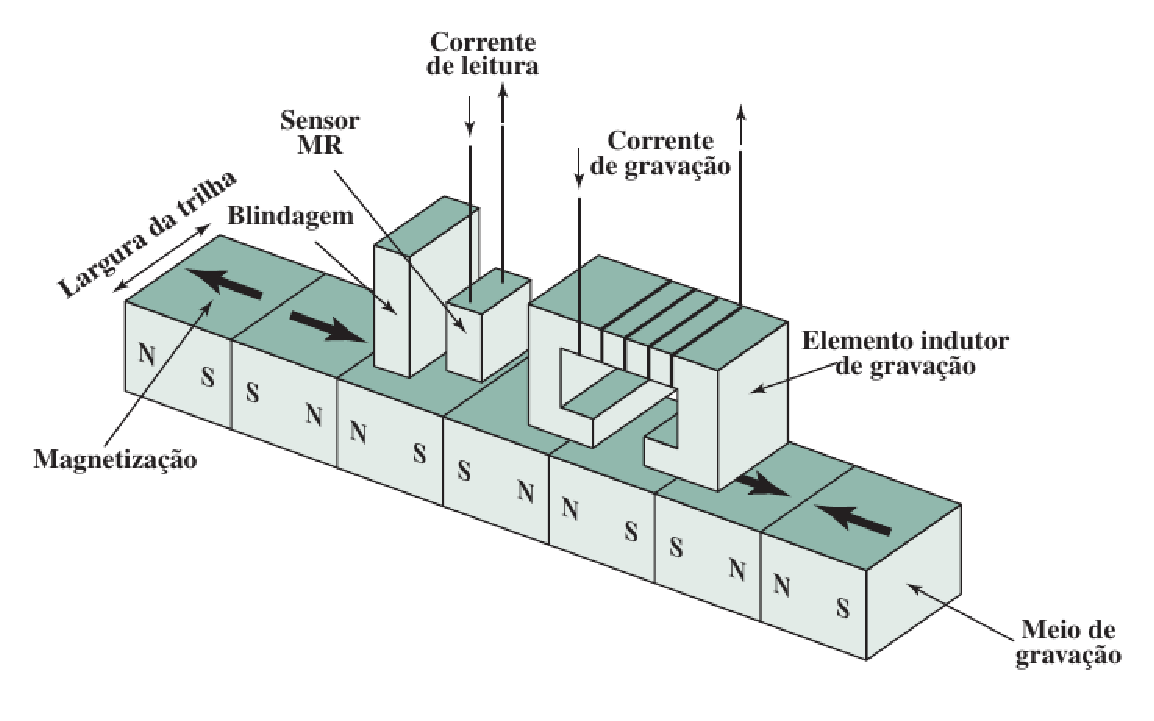
\includegraphics[width=0.45\textwidth]{figs/cabeca-gravacao-leitura}
	\end{figure}
\end{slide}

\begin{slide}{Organização dos dados}
	\begin{itemize}
	%	\item Organização dos dados:
	%		\begin{itemize}
				\item Trilhas: 
					\begin{itemize}
						\item Anéis concêntricos
						\item Mesma largura que os cabeçotes
						\item Há milhares por superfície
					\end{itemize}
				\item Intertrack gaps: 
					\begin{itemize} 
						\item Separação entre trilhas, com objetivo de redução de \emph{erros}
						\item \emph{Desalinhamento de cabeçote}
						\item \emph{Interferência de campos magnéticos}
					\end{itemize}
				\item Setores: 
					\begin{itemize}
						\item Unidades de transferência de dados
						\item Há centenas por trilha
						\item Tamanhos fixos ou variáveis (512 bytes é usado na maioria dos sistemas)
					\end{itemize}
				\item Intersector gaps: separação entre setores
	%		\end{itemize}
	\end{itemize}
\end{slide}

\begin{slide}{Organização dos dados}
	\begin{itemize}
		\item Organização dos dados (https://www.youtube.com/watch?v=NtPc0jI21i0)
			\begin{figure}[h]
				\centering
				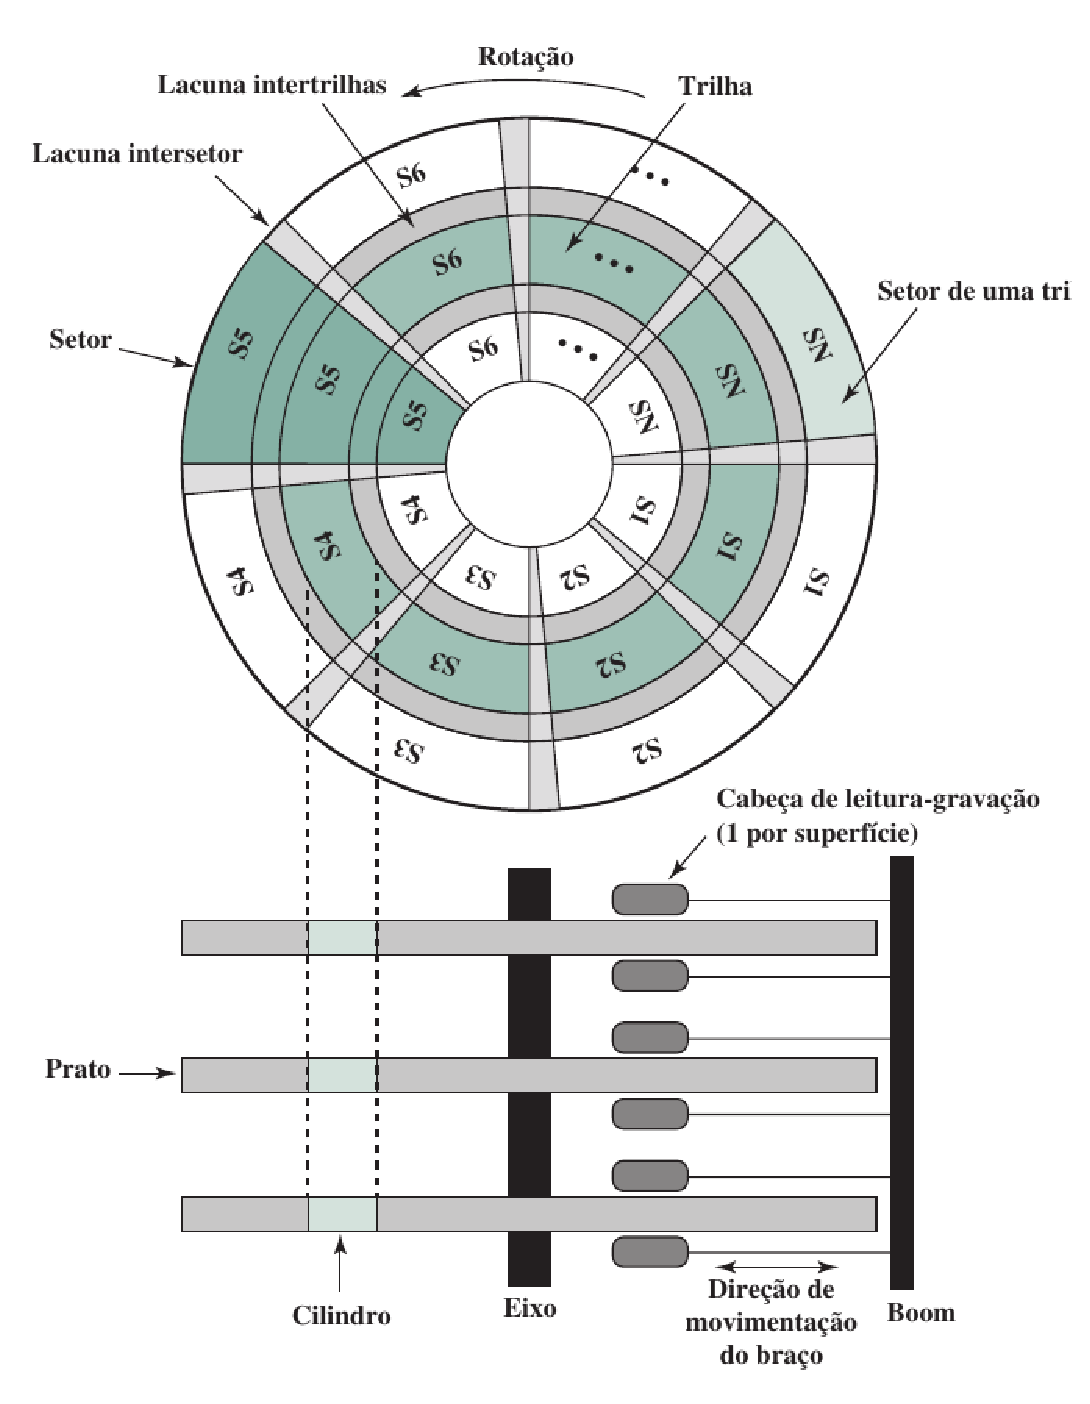
\includegraphics[width=0.38\textwidth]{figs/layout-disco}
				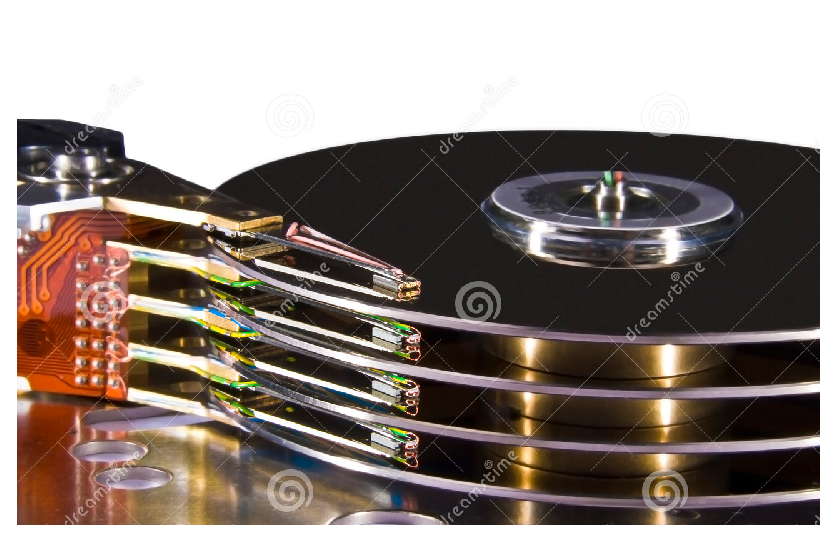
\includegraphics[width=0.55\textwidth]{figs/hd}
			\end{figure}
	\end{itemize}
\end{slide}

\begin{slide}{Organização dos dados}
	\begin{itemize}
		\item A velocidade linear varia com a distância em relação ao centro do disco
		\item Para garantir a mesma taxa de bits, o espaçamento entre estes diminui quanto mais externa for a trilha (velocidade angular constante - CAV)
			\begin{itemize}
				\item Vantagem: acesso a blocos de dados diretamente por trilha e setor
				\item Desvantagem: trilhas mais externas possuem menor densidade de bits
				\item Solução: densidade variável em cada trilha (resulta em circuitos mais complexos)
			\end{itemize}
		\item Gravação em múltiplas zonas (MZR):
			\begin{itemize}
				\item A superfície é dividida em zonas concêntricas (tipicamente 16)
				\item Cada zona contém um número de trilhas contíguas (milhares)
				\item Em cada zona, o número de bits por trilha é constante
				\item Zonas mais distantes do centro contém mais bits (mais setores)
				\item A densidade de bits é aproximadamente constante em toda a superfície do disco
			\end{itemize}
	\end{itemize}
\end{slide}

\begin{slide}{Organização dos dados}
	\begin{itemize}
		\item Comparação entre CAV e MZR
			\begin{figure}[h]
				\centering
				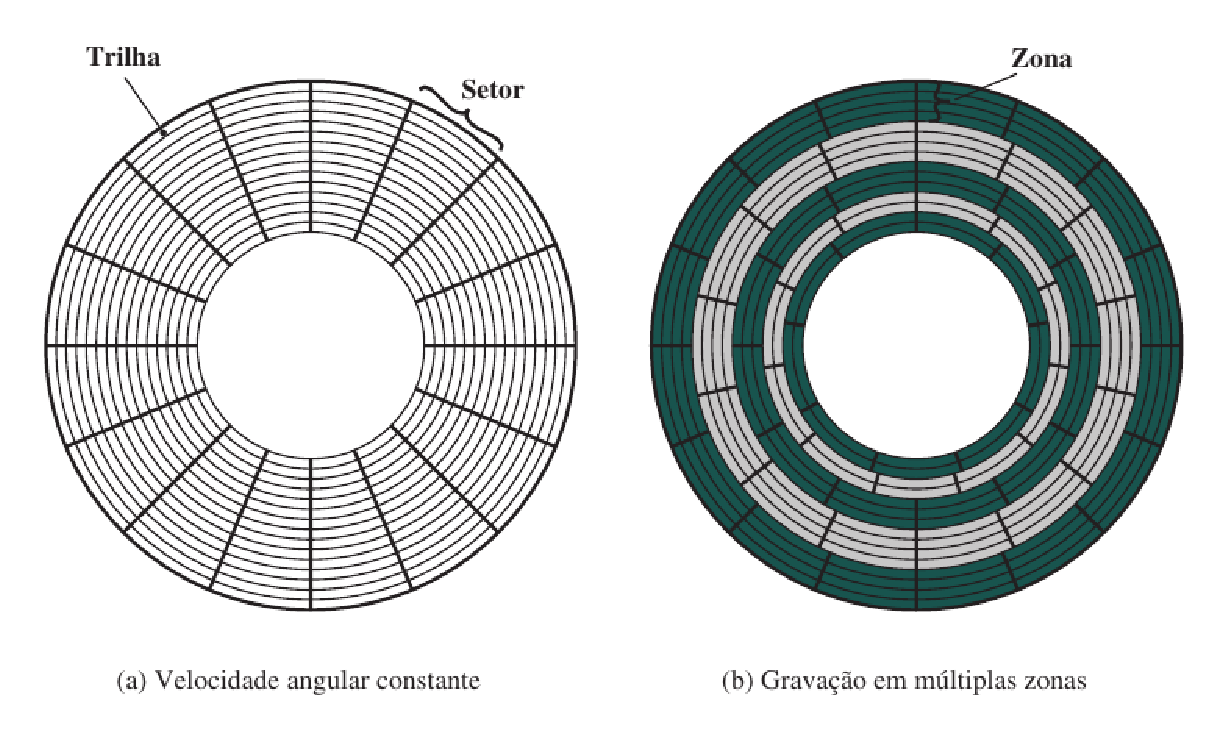
\includegraphics[width=0.8\textwidth]{figs/comparacao-layout}
			\end{figure}
	\end{itemize}
\end{slide}

\begin{slide}{Formatação}
	\begin{itemize}
		\item É necessário localizar/identificar cada setor em uma trilha
		\item Marcadores de início de trilha e de início e fim de setores
		\item Dados de formatação do disco (transparentes para o usuário)
		\item Exemplo:
			\begin{itemize}
				\item Cada trilha: 30 setores
				\item Cada setor: 600 bytes (total), 512 bytes (dados)
			\end{itemize}
	\end{itemize}
			\begin{figure}[h]
				\centering
				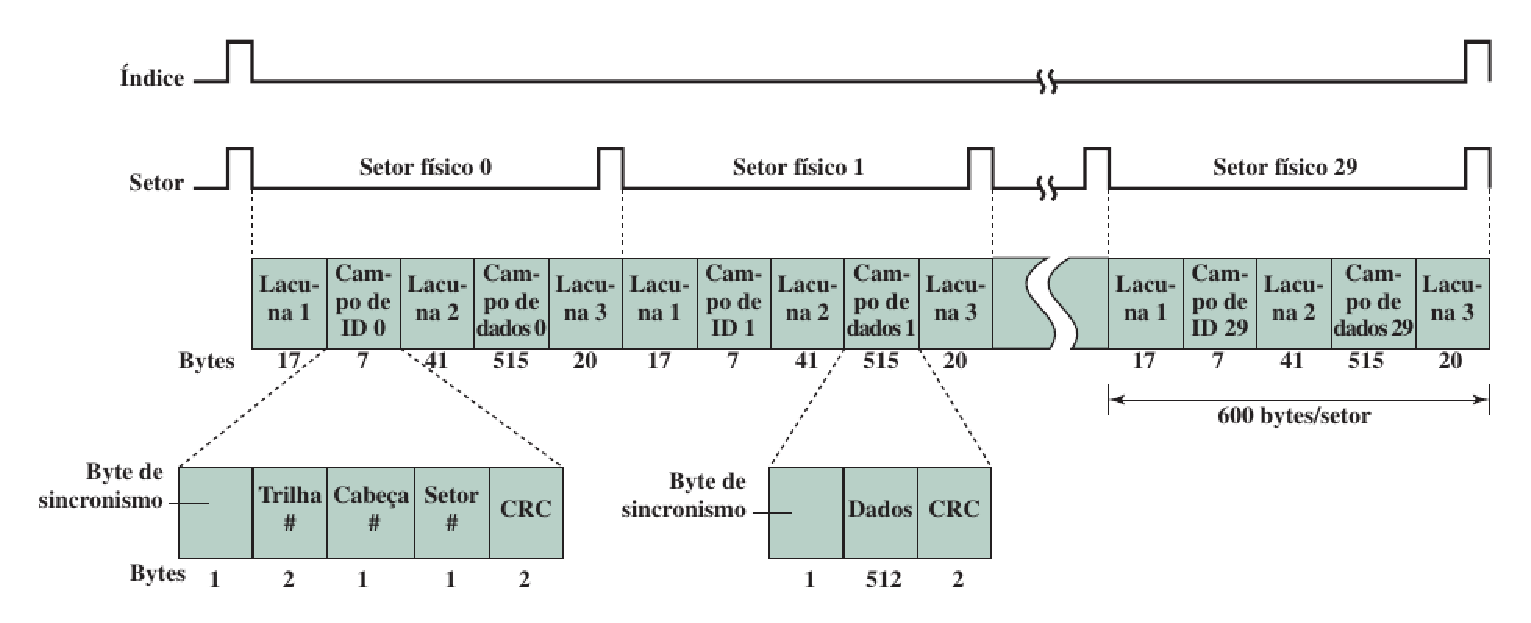
\includegraphics[width=0.7\textwidth]{figs/formato-winchester}
			\end{figure}
\end{slide}

\begin{slide}{Características físicas}
	\begin{itemize}
		\item Principais características físicas
			\begin{figure}[h]
				\centering
				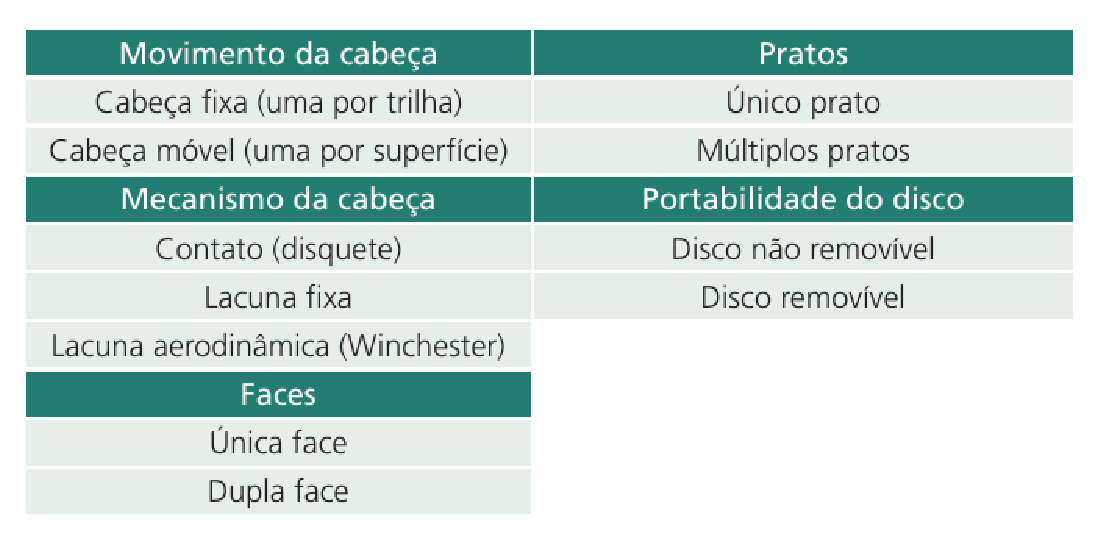
\includegraphics[width=0.7\textwidth]{figs/caracteristicas-fisicas-disco}
			\end{figure}
	\end{itemize}
\end{slide}

\begin{slide}{Parâmetros de desempenho}
	\begin{itemize}
		\item Tempo de busca (\emph{seek time}): tempo necessário para posicionamento da cabeça na trilha correta
		\item Latência (\emph{rotational latency}): tempo para alcançar o início do setor
		\item Tempo de acesso (\emph{access time}): tempo de busca + latência
		\item Tempo de transferência de dados (\emph{transfer time})
			\begin{figure}[h]
				\centering
				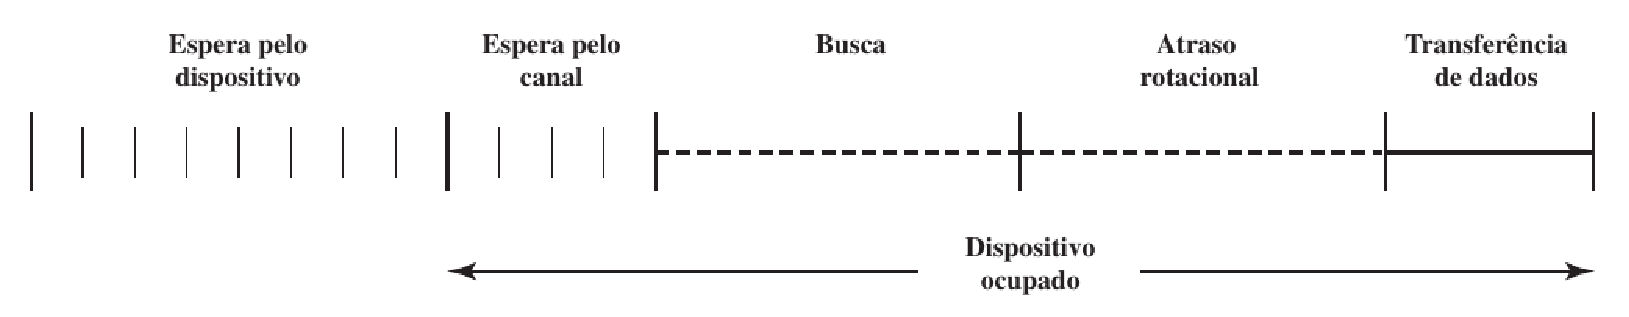
\includegraphics[width=0.8\textwidth]{figs/temporizacao}
			\end{figure}
		\item Tempo total
			\begin{equation*}
				T_\text{total} = T_\text{busca} + T_\text{latência} + T_\text{transferência} = T_\text{busca} + \frac{1}{2r} + \frac{b}{rN}
			\end{equation*}
			onde $r$, $b$, e $N$ representam a velocidade de rotação, o número de bytes a ser transferido, e o número de bytes em uma trilha, respectivamente.
	\end{itemize}
\end{slide}
\begin{slide}{Parâmetros de desempenho}
	\begin{itemize}
		\item Parâmetros típicos
			\begin{figure}[h]
				\centering
				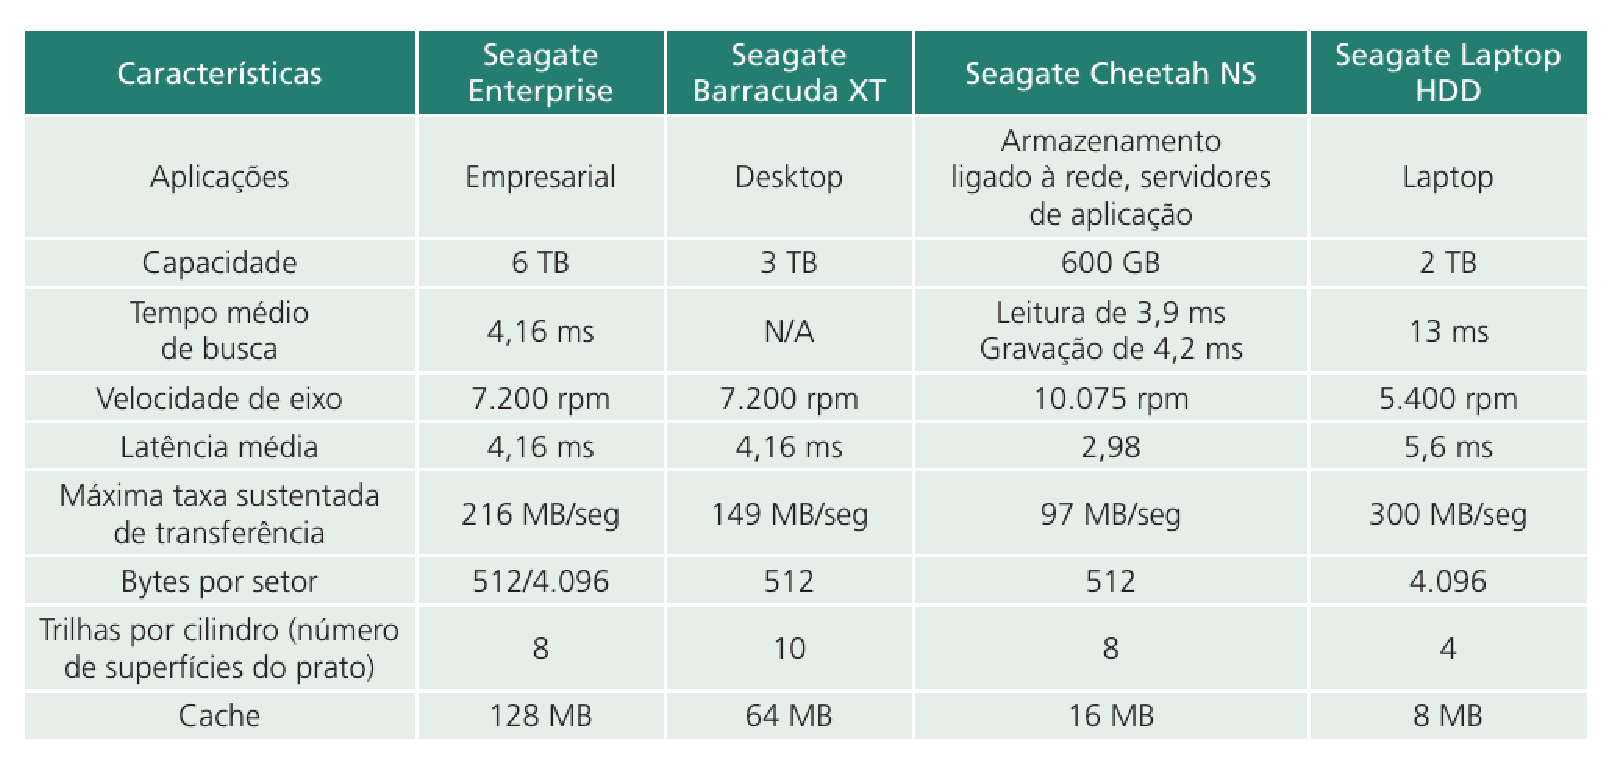
\includegraphics[width=0.9\textwidth]{figs/parametros-drive}
			\end{figure}
	\end{itemize}
\end{slide}

\section[slide=true]{RAID}
\begin{slide}{RAID - razões e princípios}
	\begin{itemize}
		\item O desempenho dos discos é menor, se comparado a processadores e memória principal
		\item Pode-se obter melhoria mediante o acréscimo de elementos operando em paralelo
		\item RAID (\emph{redundant array of independent disks}):
			\begin{itemize}
				\item Conjunto de discos físicos visto pelo sistema operacional como um único drive lógico
				\item Distribuição de dados no arranjo de drives segundo um esquema conhecido como \emph{striping}
				\item Permite o armazenamento de informação de paridade para proteção contra falhas de disco
				\item Tipos: \textbf{RAID 0}, \textbf{RAID 1}, RAID 2, RAID 3, RAID 4, \textbf{RAID 5}, \textbf{RAID 6}
			\end{itemize}
	\end{itemize}
\end{slide}

\begin{slide}{RAID nível 0}
	\begin{itemize}
		\item Não inclui redundância para melhoramento de desempenho
		\item O disco lógico é dividido em \emph{strips} (blocos físicos, setores ou alguma outra unidade)
		\item Os \emph{strips} são mapeados em discos consecutivos no arranjo RAID
		\item \emph{Stripe}: conjunto lógico de \emph{strips} que são mapeados cada um em um elemento do arranjo de discos
		\item A leitura de \emph{strips} consecutivas pode ser feita em paralelo
		\item Melhor taxa de transferência de dados, e aumento da taxa de requisição
			\begin{figure}[h]
				\centering
				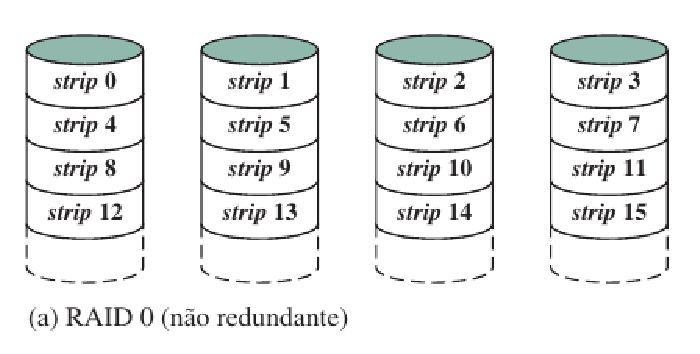
\includegraphics[width=0.55\textwidth]{figs/raid0}
			\end{figure}
	\end{itemize}
\end{slide}

\begin{slide}{RAID nível 0}
	\begin{itemize}
		\item \emph{Software} de gerenciamento de arranjo
			\begin{figure}[h]
				\centering
				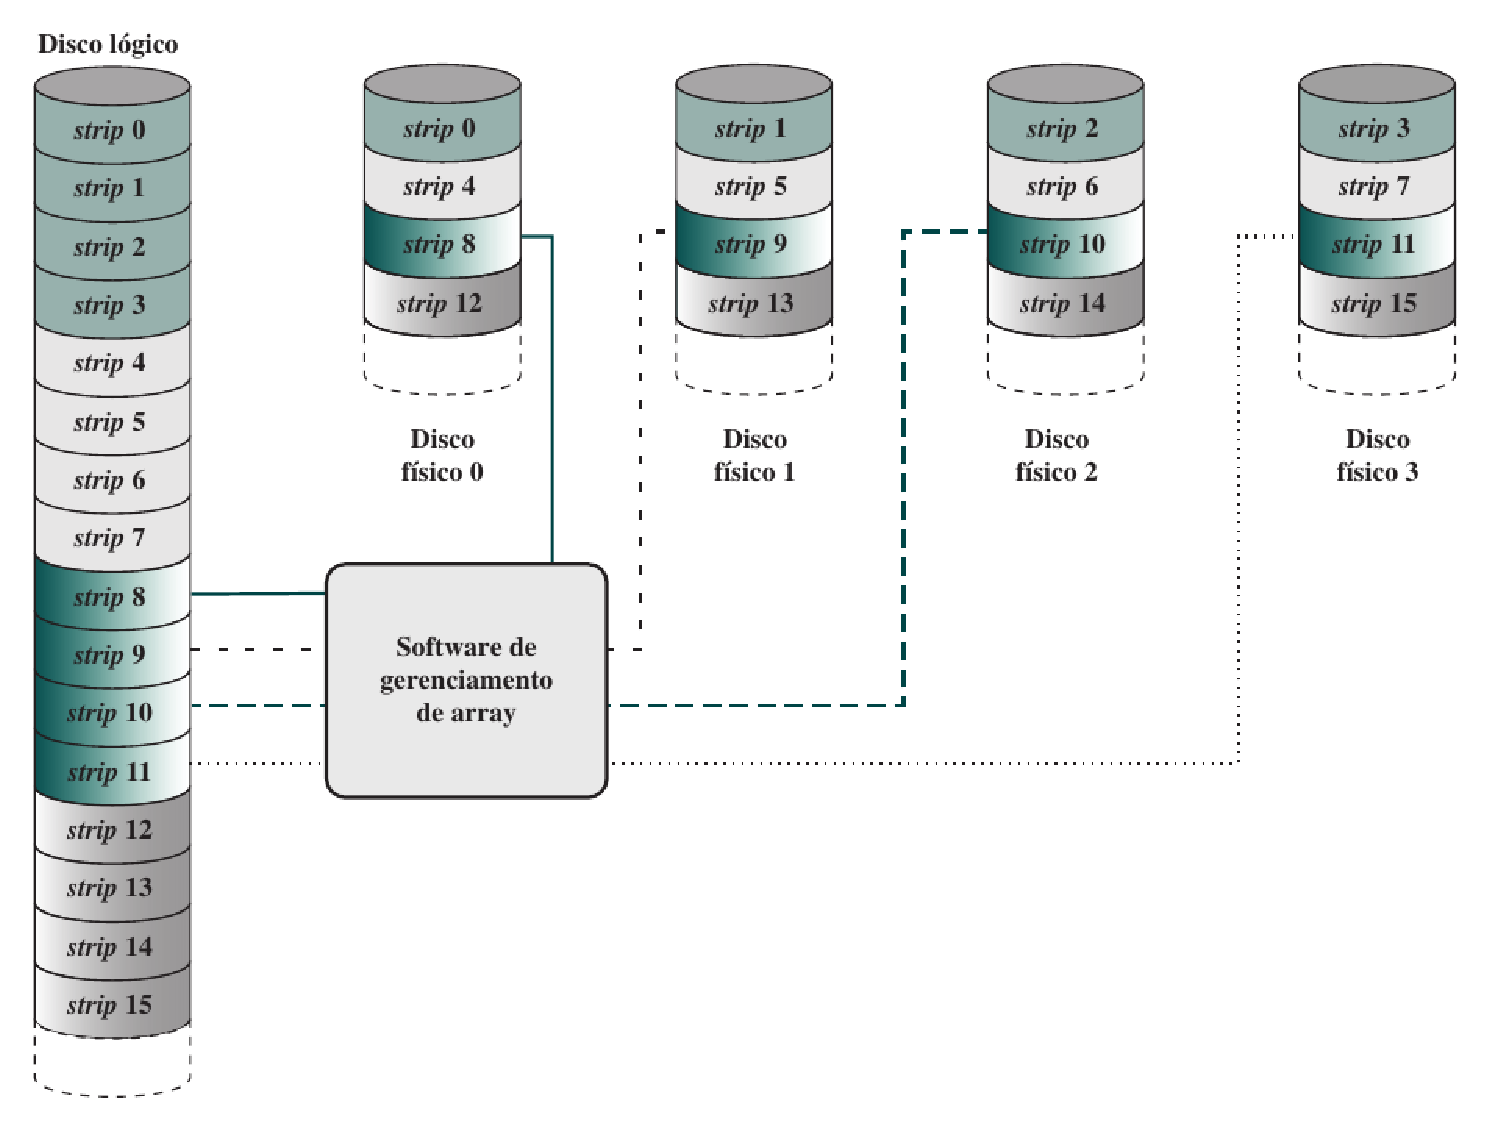
\includegraphics[width=0.65\textwidth]{figs/mapeamento}
			\end{figure}
	\end{itemize}
\end{slide}

\begin{slide}{RAID nível 1}
	\begin{itemize}
		\item Redundância por duplicação dos dados (espelhamento)
			\begin{figure}[h]
				\centering
				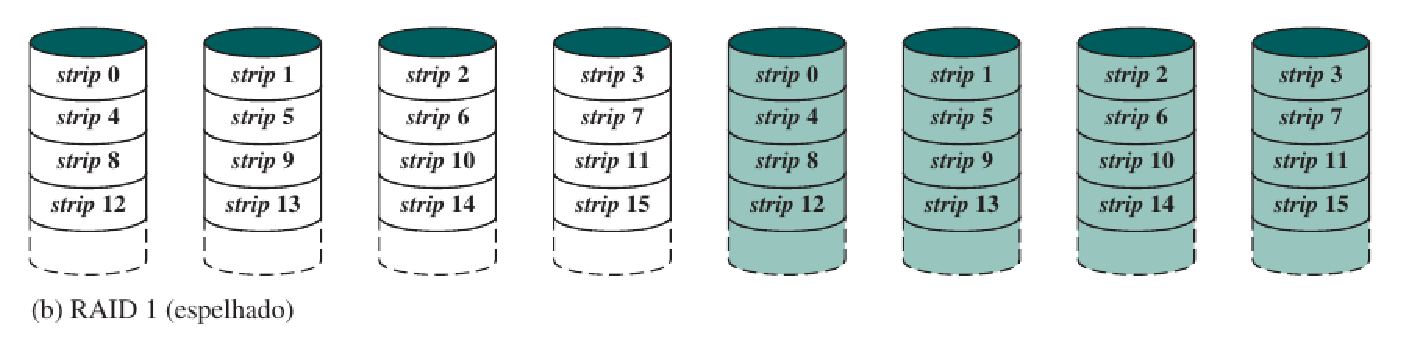
\includegraphics[width=0.75\textwidth]{figs/raid1}
			\end{figure}
		\item Características:
			\begin{itemize}
				\item Uma requisição pode ser atendida pelo disco que tiver menor tempo de acesso
				\item Uma escrita deve ser atualizada em todas as \emph{strips} correspondentes (desempenho geral é o da escrita mais lenta)
				\item Recuperação de dados em caso de falha é simples
				\item Custo é a principal desvantagem 
				\item Normalmente usado para armazenar arquivos do sistema e dados críticos
			\end{itemize}
	\end{itemize}
\end{slide}

\begin{slide}{RAID nível 2}
	\begin{itemize}
		\item Usa técnica de acesso paralelo (braços e cabeçotes sincronizados em todos os discos)
		\item \emph{Strips} pequenos (\emph{byte} ou palavra)
		\item Adota código de Hamming (SEC-DED)
		\item Número de discos de redundância é proporcional ao logaritmo do número de discos de dados
		\item Não é implementado na prática (custo associado é desnecessário)
	\end{itemize}

			\begin{figure}[h]
				\centering
				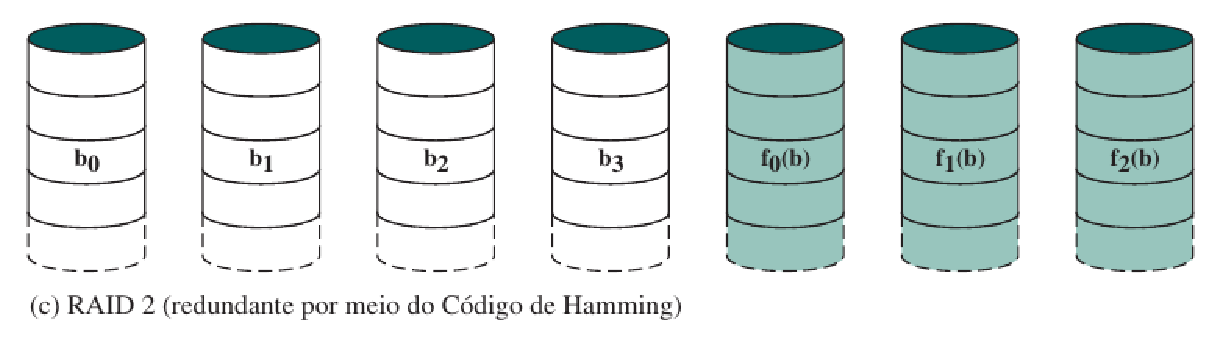
\includegraphics[width=0.75\textwidth]{figs/raid2}
			\end{figure}
\end{slide}

\begin{slide}{RAID nível 3}
	\begin{itemize}
		\item Organização semelhante ao RAID 2
		\item Usa apenas um disco para paridade, não importando o número de discos de dados
	        \item Adota técnica de acesso paralelo (como no RAID 2)
		\item Em lugar de código correto de erro, calcula bit de paridade para bits na mesma posição em todos os discos de dados
		\item Em caso de falha de um drive, disco de paridade é usado para restaurar o drive perdido
			\begin{figure}[h]
				\centering
				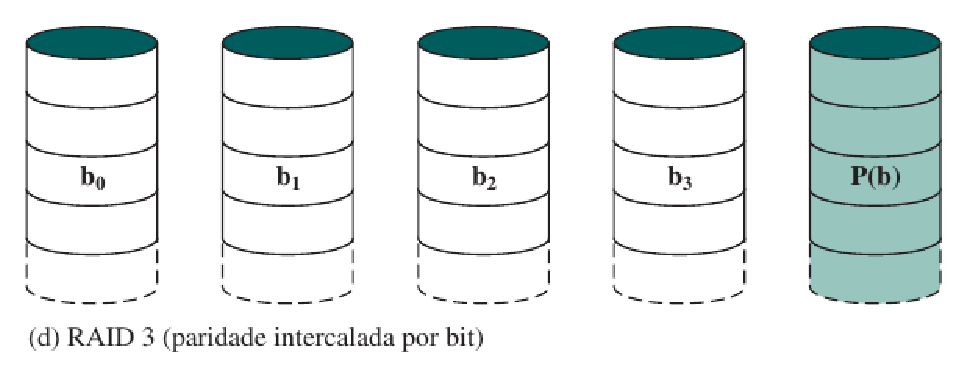
\includegraphics[width=0.75\textwidth]{figs/raid3}
			\end{figure}
	\end{itemize}
\end{slide}

\begin{slide}{RAID nível 4}
	\begin{itemize}
		\item Usa técnica de acesso independente
		\item Mais adequado a demandas onde o atendimento de requisições simultâneas é prioritário
		\item Adota \emph{strips} maiores
		\item Paridade por blocos \emph{strips}
		\item Penalidade para escrita para conjunto de dados pequeno
		\item Gargalo associado à escrita no disco de paridade
			\begin{figure}[h]
				\centering
				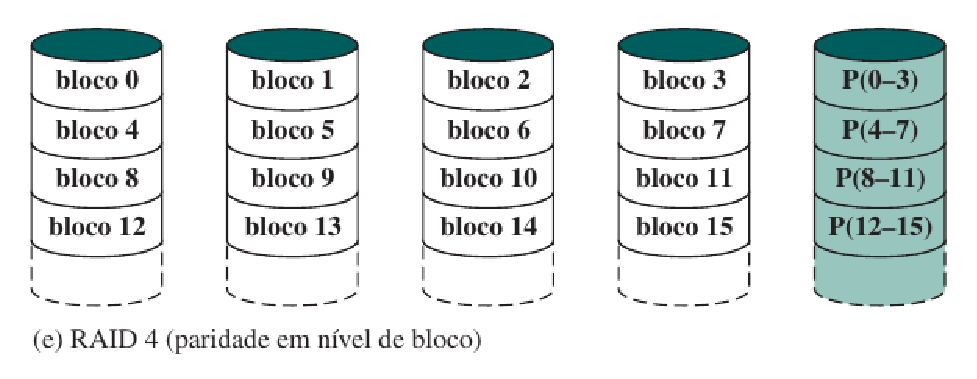
\includegraphics[width=0.75\textwidth]{figs/raid4}
			\end{figure}
	\end{itemize}
\end{slide}

\begin{slide}{RAID nível 5}
	\begin{itemize}
		\item Esquema semelhante ao do RAID 4
		\item \emph{Strips} de paridade distribuídas nos discos
		\item Reduz gargalo em relação ao disco de paridade
			\begin{figure}[h]
				\centering
				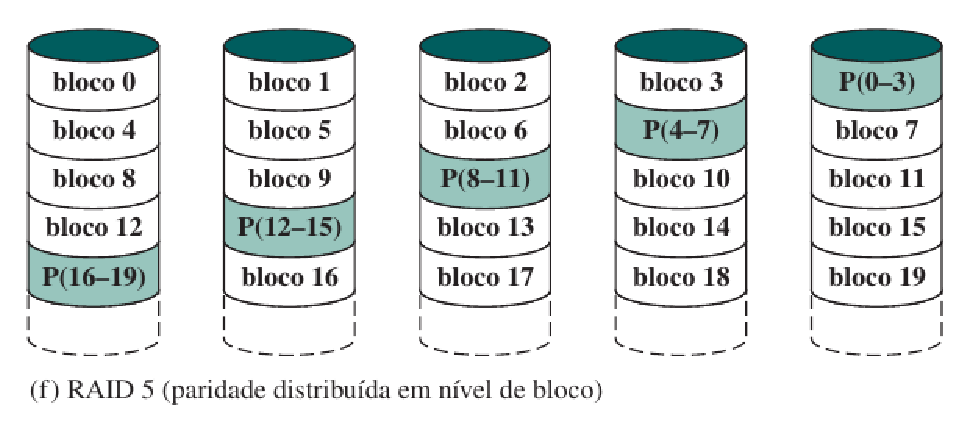
\includegraphics[width=0.75\textwidth]{figs/raid5}
			\end{figure}
	\end{itemize}
\end{slide}

\begin{slide}{RAID nível 6}
	\begin{itemize}
		\item Semelhante ao RAID 5
		\item Usa dois \emph{strips} de verificação de dados por \emph{stripe}
			\begin{itemize}
				\item Algoritmo baseado no OU-Exclusivo
				\item Algoritmo independente (diferente)
			\end{itemize}
		\item Proteção contra falha de até dois discos
		\item Penalidade de escrita mais alta que em RAID 5
		\item Desempenho em leitura comparável a RAID 5
			\begin{figure}[h]
				\centering
				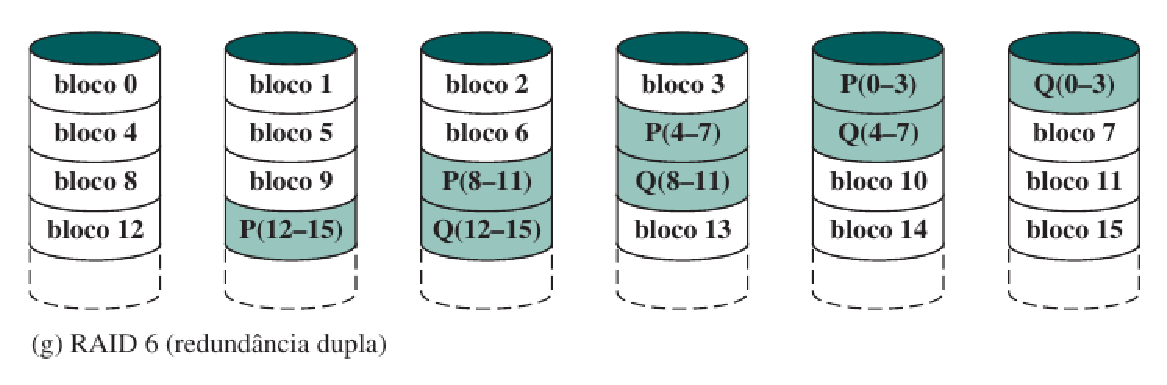
\includegraphics[width=0.75\textwidth]{figs/raid6}
			\end{figure}
	\end{itemize}
\end{slide}

\section[slide=true]{Drives de estado sólido}
\begin{slide}{Drives de estado sólido}
	\begin{itemize}
		\item Conhecidos pela sigla SSD (do inglês, \emph{solid state drive})
		\item Utilizados como complemento ou substituição aos HDDs (do inglês, \emph{hard disk drives})
		\item Uso em memória secundária ou externa
		\item É implementado por meio de semicondutores
		\item Vantagens:
			\begin{itemize}
				\item Melhor desempenho
				\item Maior durabilidade (menor suscetibilidade à vibração e choques físicos)
				\item Maior vida útil
				\item Menor consumo de energia
			\end{itemize}
		\item Desvantagens: 
			\begin{itemize}
				\item Maior custo por bit
				\item Desaceleração de desempenho (memória virtual vs. memória flash)
				\item ``Morte'' da memória flash (aproximadamente 100.000 gravações)
			\end{itemize}
	\end{itemize}
\end{slide}

\begin{slide}{Comparação SSD vs. HDD}
	\begin{itemize}
		\item Algumas características comparadas (atualizar)
			\begin{figure}
				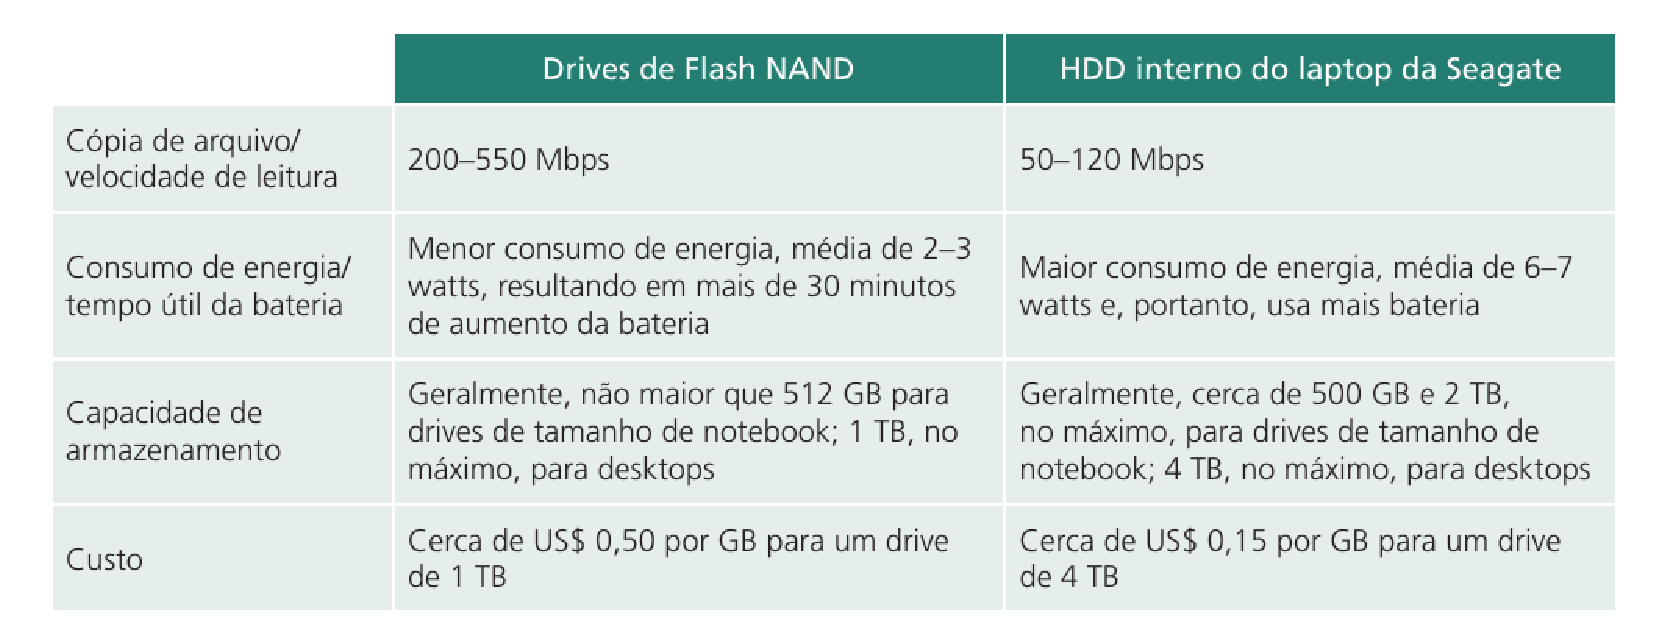
\includegraphics[width=\textwidth]{figs/tab6-5}
			\end{figure}
	\end{itemize}
\end{slide}
\begin{slide}{Arquitetura de um SSD}
	\begin{itemize}
		\item Elementos de um drive de estado sólido
			\begin{figure}
				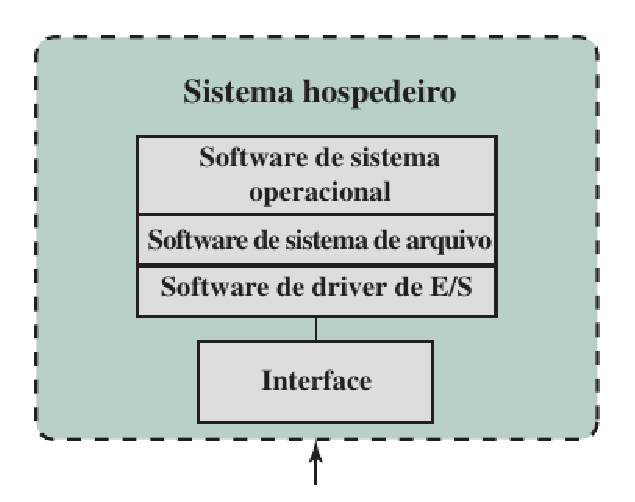
\includegraphics[width=0.30\textwidth]{figs/ssd1}
				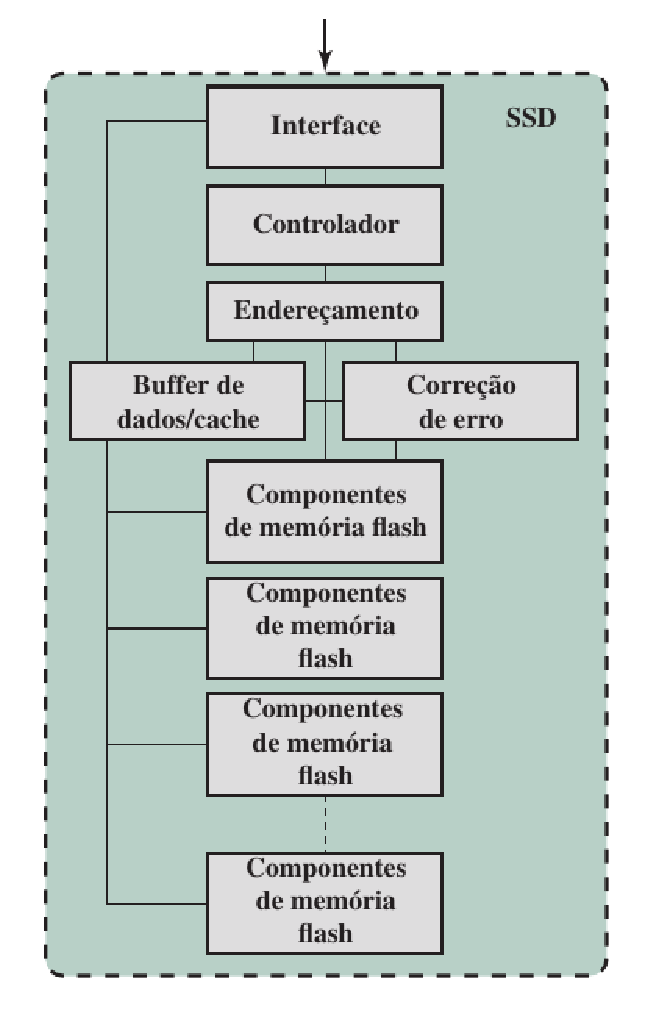
\includegraphics[width=0.30\textwidth]{figs/ssd2}
			\end{figure}
	\end{itemize}
\end{slide}

\section[slide=true]{Memória óptica}
\begin{slide}{Discos ópticos}
	\begin{itemize}
		\item Panorama geral
			\begin{figure}
				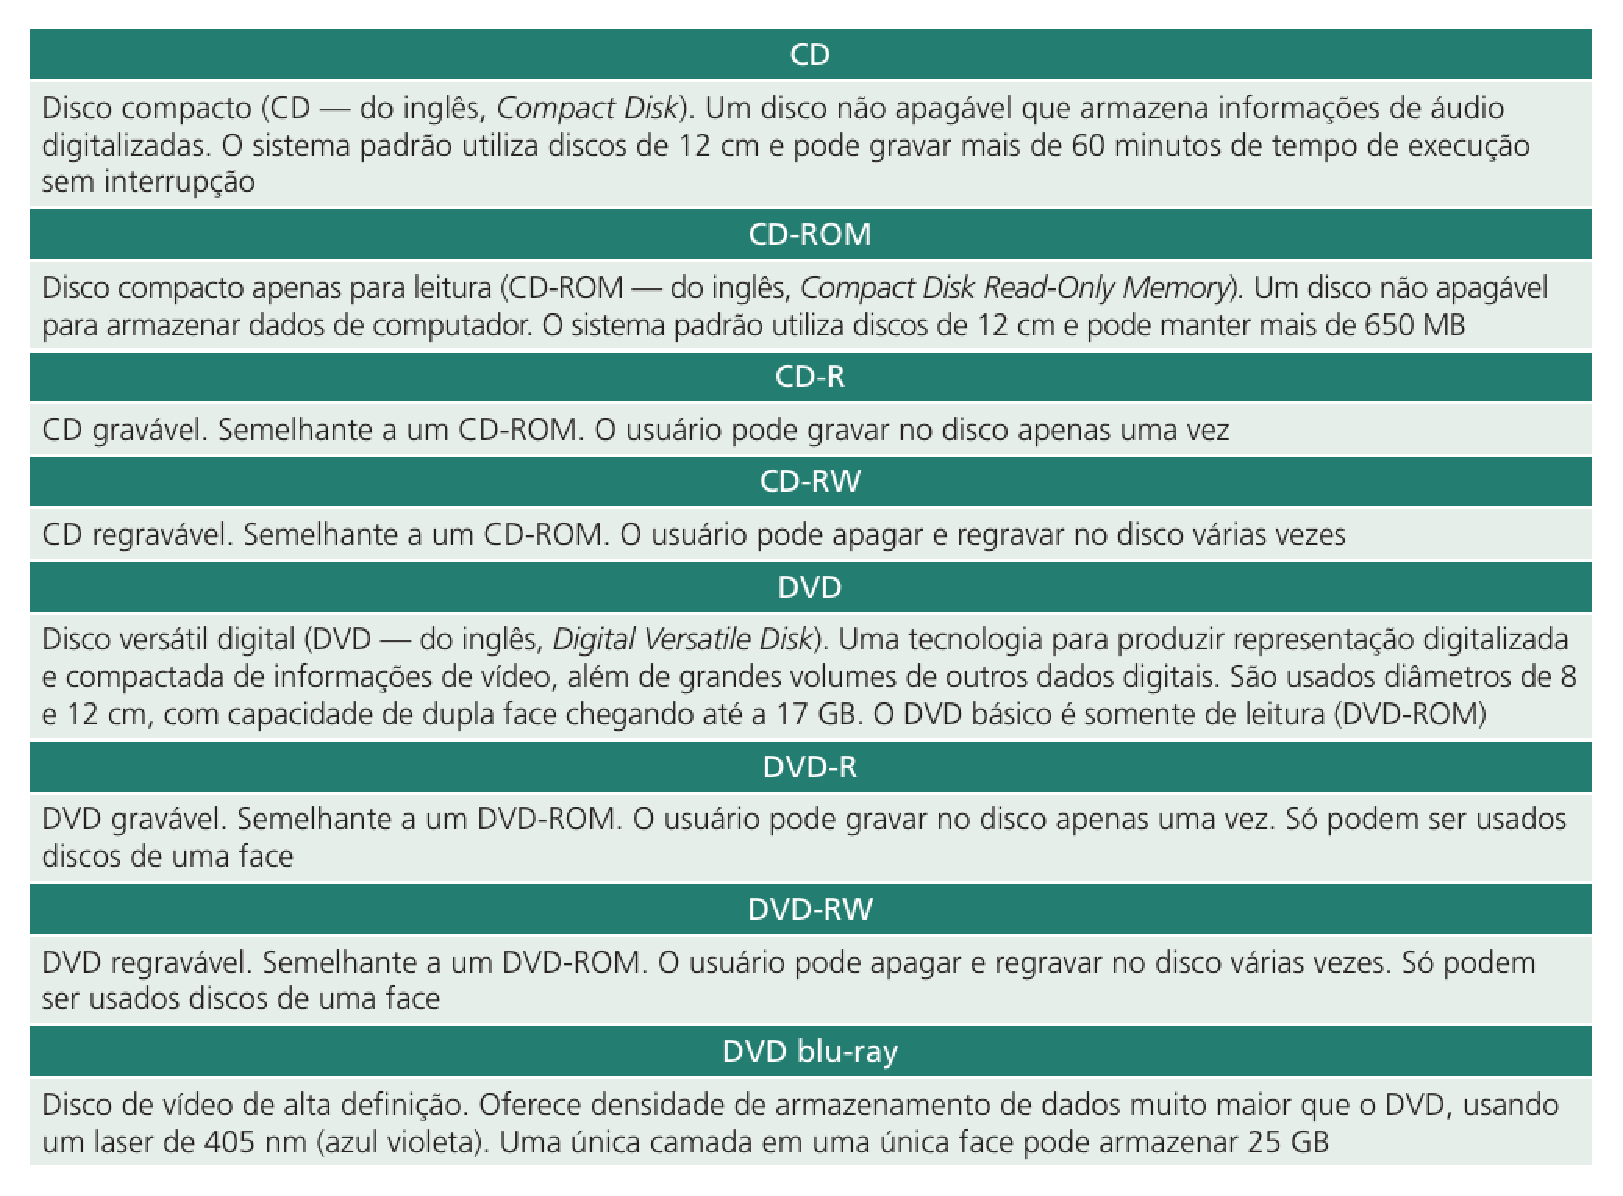
\includegraphics[width = 0.7\textwidth]{figs/dopticos}
			\end{figure}
	\end{itemize}
\end{slide}
\begin{slide}{Operação do CD}
	\begin{itemize}
		\item Transmissão e recepção de lasers
			\begin{figure}
				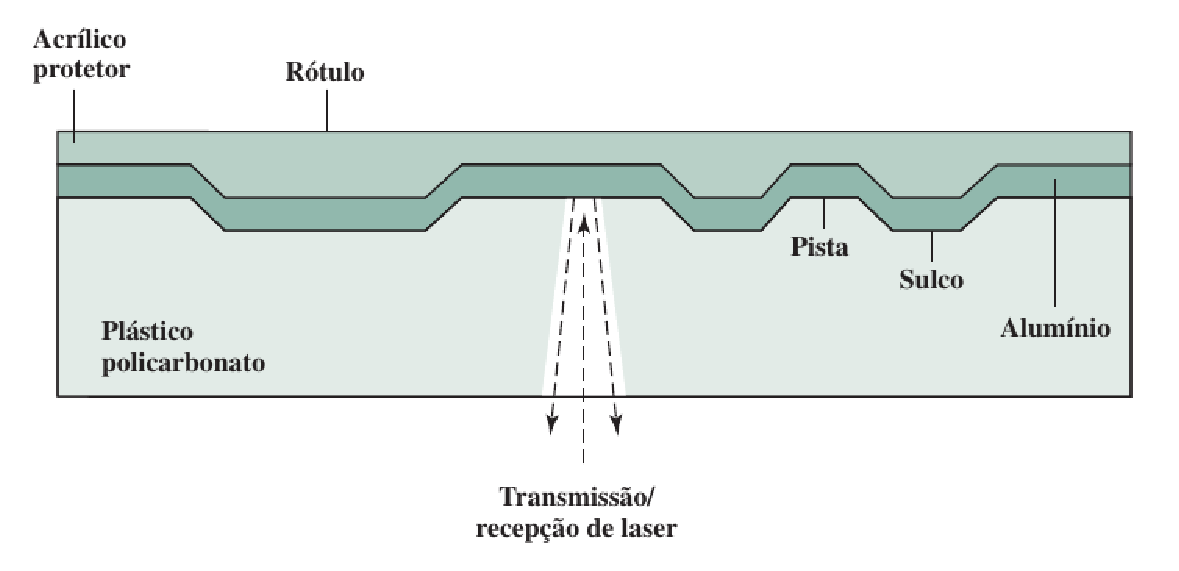
\includegraphics[width = 0.9\textwidth]{figs/opt-cd}
			\end{figure}
	\end{itemize}
\end{slide}
\begin{slide}{Organização de dados}
	\begin{itemize}
		\item Formato de bloco do CD-ROM
			\begin{figure}
				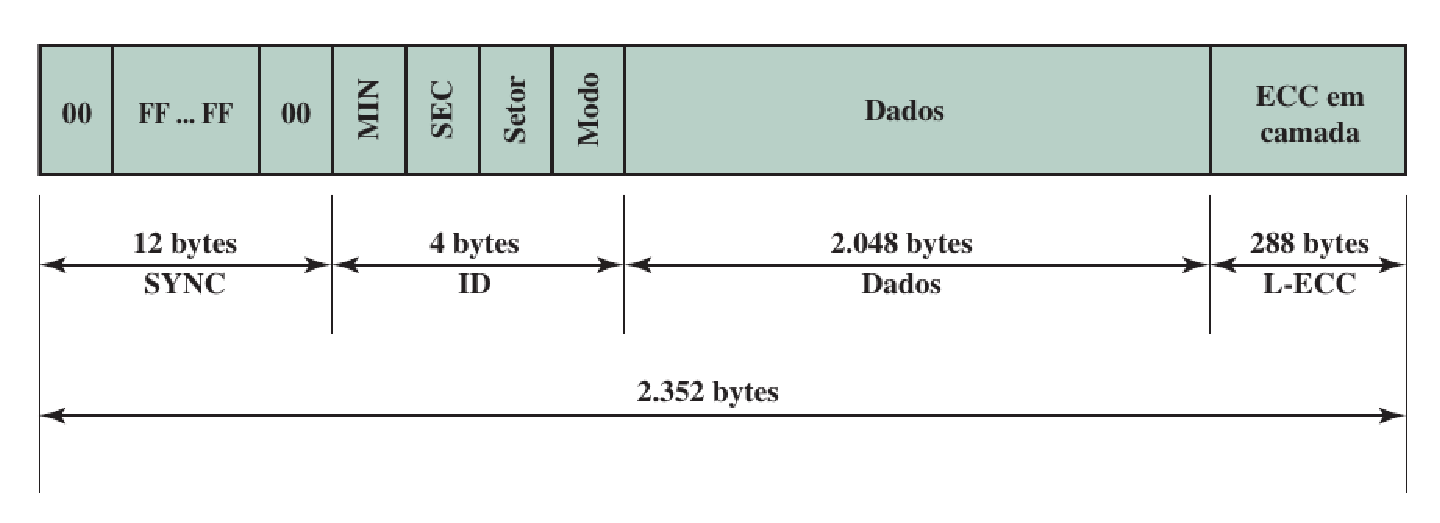
\includegraphics[width = 0.9\textwidth]{figs/opt-cd-bloco}
			\end{figure}
	\end{itemize}
\end{slide}
\begin{slide}{CD e DVD}
	\begin{itemize}
		\item Elementos de comparação
			\begin{figure}
				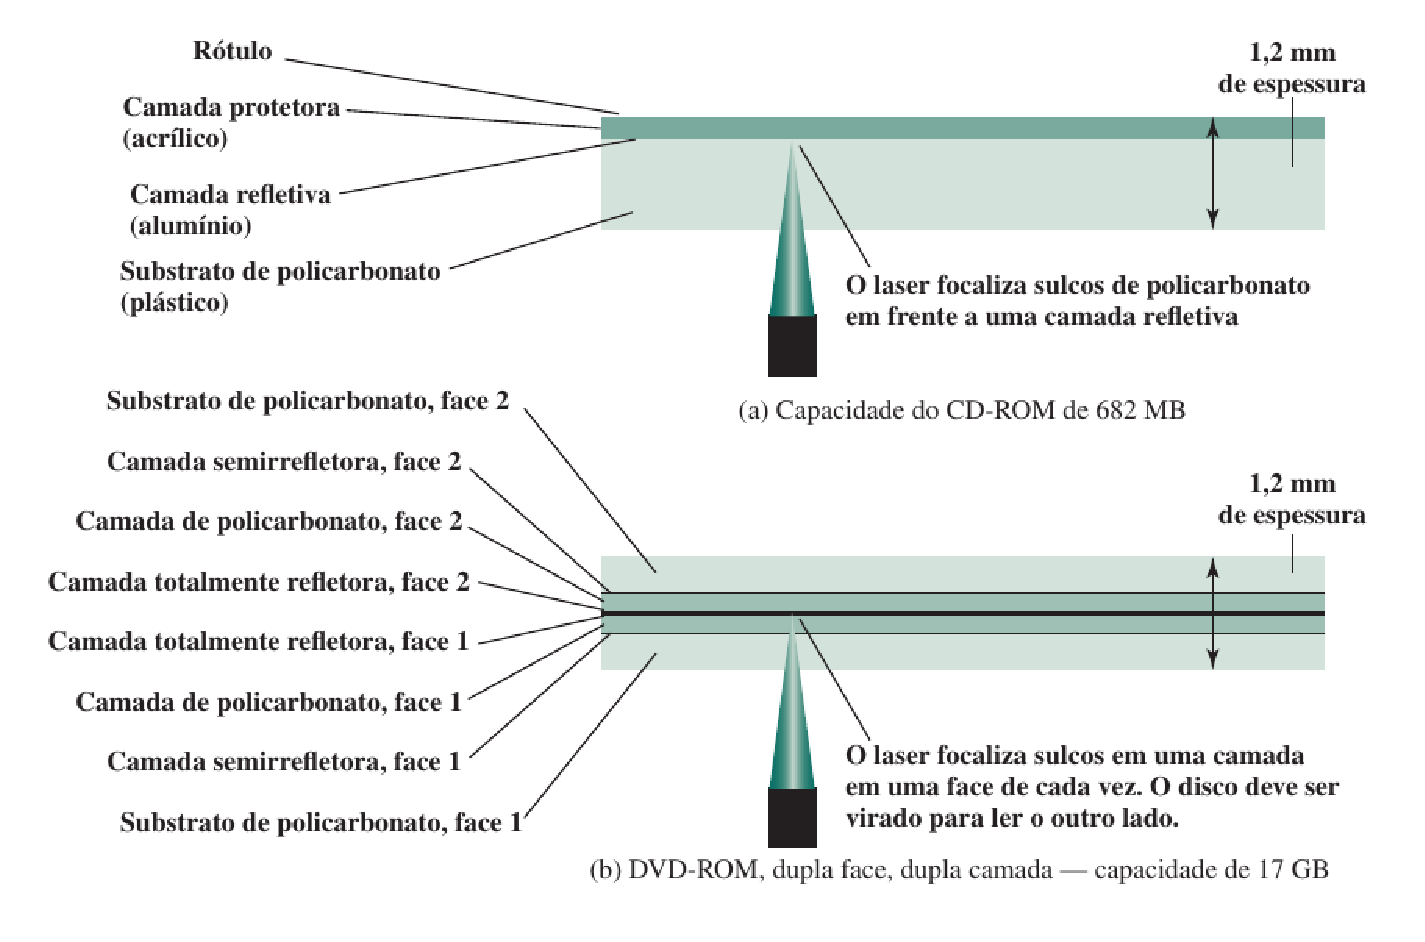
\includegraphics[width = 0.7\textwidth]{figs/opt-cd-dvd}
			\end{figure}
	\end{itemize}
\end{slide}
\begin{slide}{CD, DVD e Blue-ray}
	\begin{itemize}
		\item Elementos de comparação
			\begin{figure}
				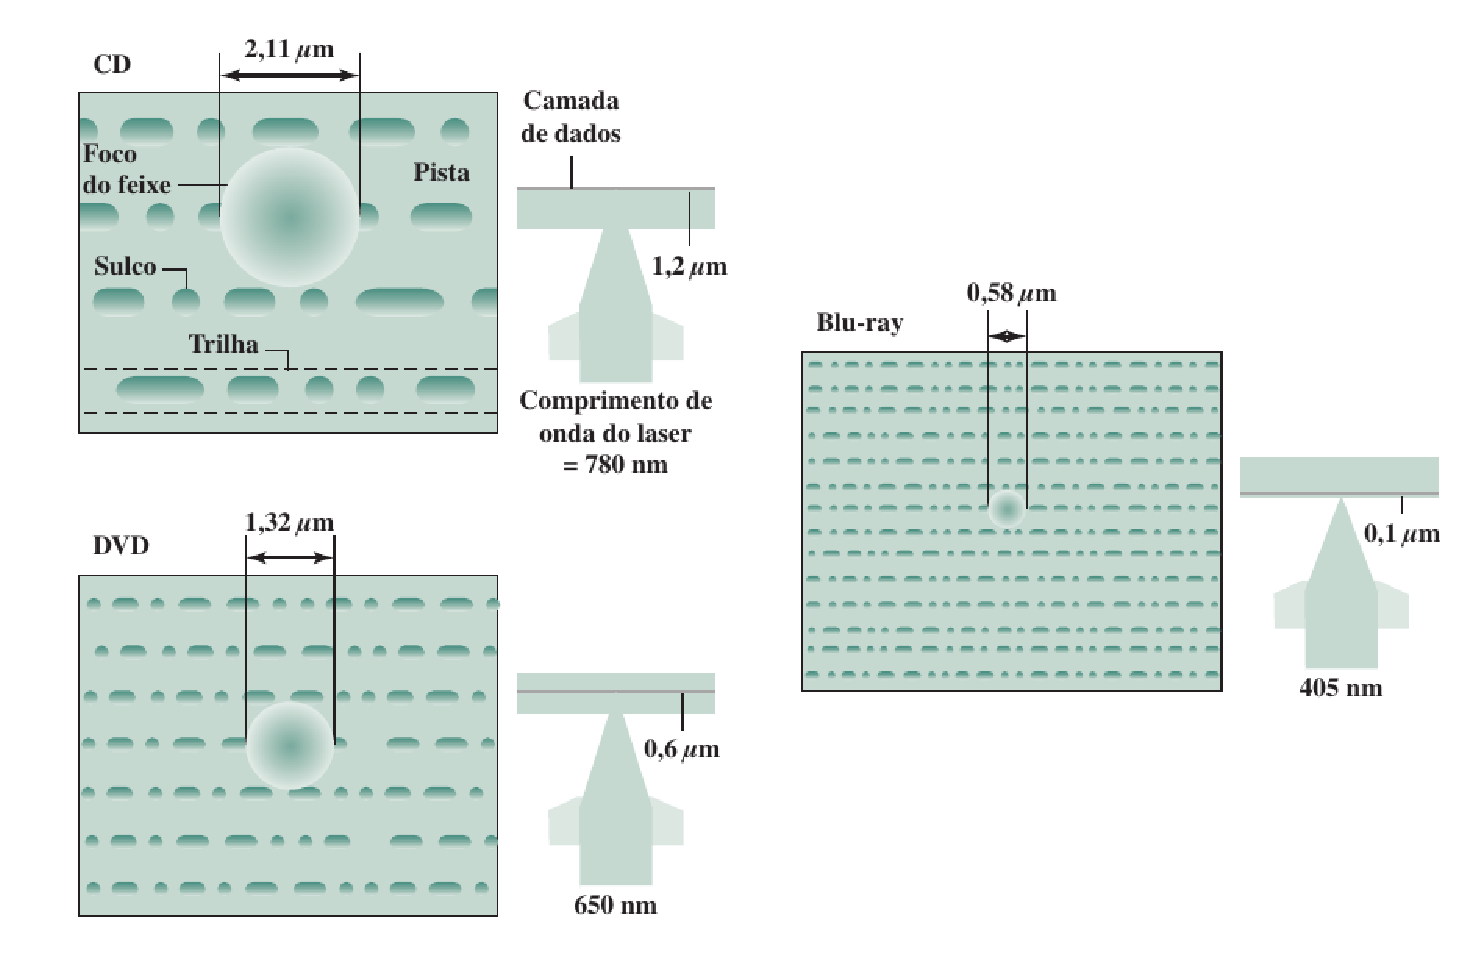
\includegraphics[width = 0.7\textwidth]{figs/opt-comp}
			\end{figure}
	\end{itemize}
\end{slide}
%\section[slide=true]{Fita magnética}
%\section[slide=true]{Memória principal semicondutora}

% \section[slide=True]{Memória flash}
% \begin{slide}{Memória flash}
% \end{slide}
%
% \section[slide=True]{Novas tecnologias de memórias de estado sólido não-voláteis}
% \begin{slide}{STT-RAM}
% \end{slide}
%
% \begin{slide}{PCRAM}
% \end{slide}
%
% \begin{slide}{ReRAM}
% \end{slide}
%
\end{document}
